\subsection{\textbf{EXP 2} - HTTP Constant Throughput}
\label{sec:experiments:results:per-experiment:02}
% Goal: To evaluate how \gls{sm} configurations behave under varying levels of load.

In the previous experiment (\cref{sec:experiments:results:per-experiment:01}), we evaluated \gls{sm} systems under maximum load. In this experiment, we evaluate these systems under varying, pre-defined levels of constant throughput. The results of these experiments aim to show how the \gls{sm} systems scale, across varying levels of load.

\subsubsection{Latency Analysis}
\label{sec:experiments:results:per-experiment:02:latency}

\begin{figure}[t]
    \centering

    \makebox[\linewidth][c]{
        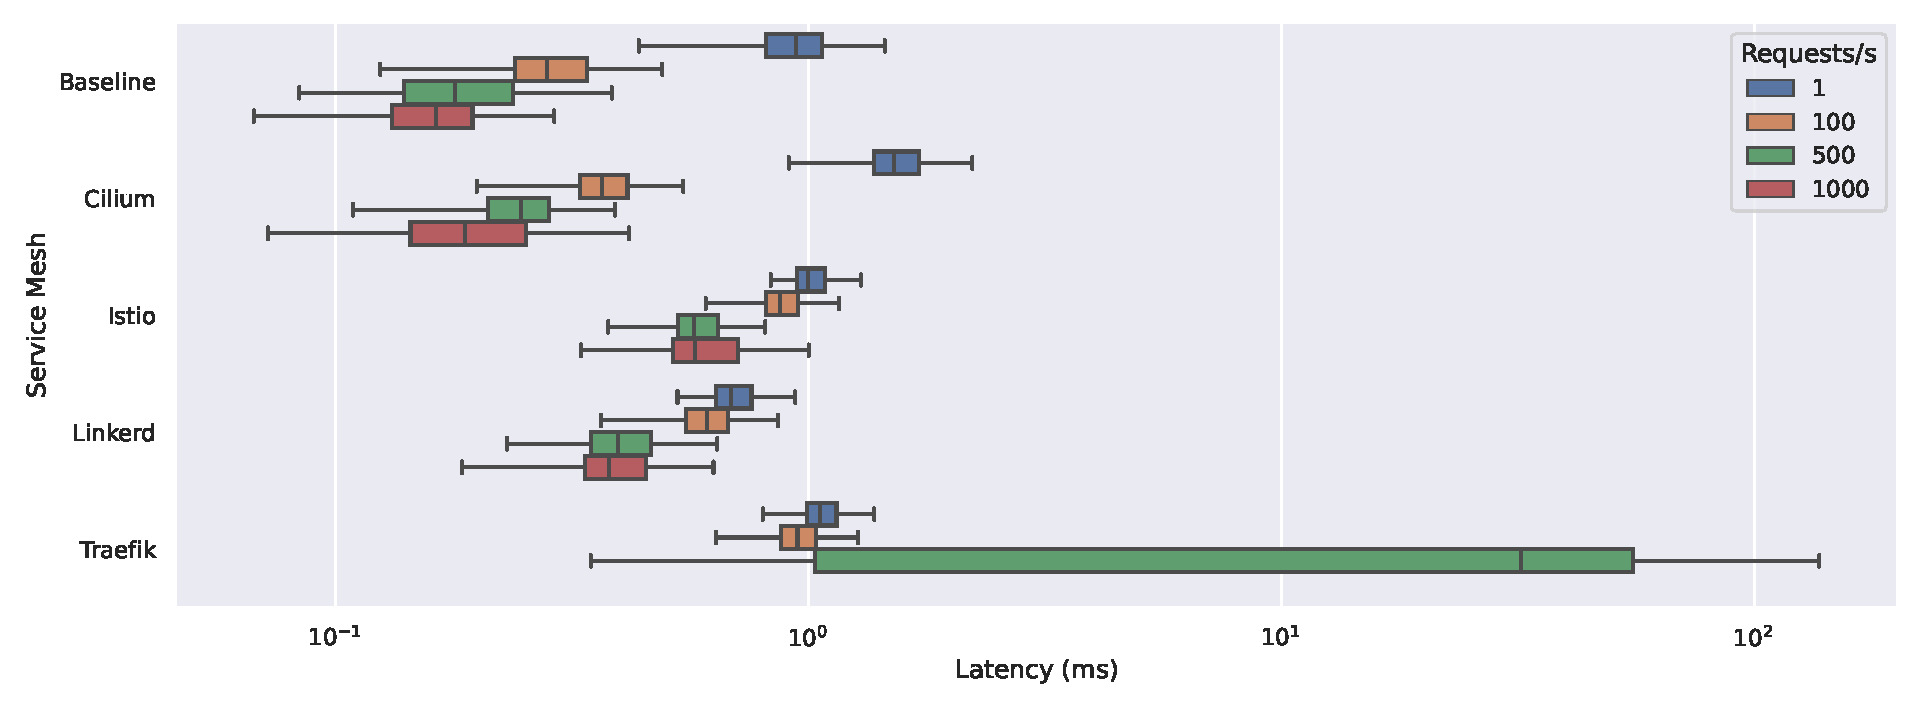
\includegraphics[width=1.2\linewidth]{5_experimental_evaluation/figures/exp-02-latency-log.pdf}
    }
    
    \caption[Experiment 2 - Distribution of observed latencies per \gls{sm} system under various levels of constant throughput.]{Distribution of observed latencies per \gls{sm} system under various levels of constant throughput on a logarithmic scale.}
    
    \label{fig:exp:02:latency-distributions}

\end{figure}


In \cref{fig:exp:02:latency-distributions} we present the latency distributions of the evaluated \gls{sm} configurations under various levels of constant throughput.  On the y-axis we present the \gls{sm} configurations and on the x-axis the latency expressed in milliseconds on a logarithmic scale. The legend on the plots display the various levels of throughput depicted on this graph and the colours that represent them.

From the figure we can derive that the latency distributions are generally close for each of the defined levels of throughput for most of the systems. This is an indication that the various levels of throughput are manageable by the evaluated configurations. This is exemplified by the average levels of throughput that these configurations were able to process as observed in our previous experiment in \cref{sec:experiments:results:per-experiment:01}. 

One exception to this, however, is that the configuration using Traefik is experiencing a significant increase in observed latencies when experiencing a constant load of 500 requests per second. Additionally, it is important to note that the results regarding 1000 requests per second have not been included in this figure, as it was unable to manage that level of throughput. As a matter of fact, it was unable to even fully sustain the constant throughput of 500 requests per second, as it only managed to process 419 requests per second in this particular experiment. This result falls in line with the observed behaviour from our previously conducted experiment, in which we evaluated these systems under maximum load. The reason that the observed throughput is even lower in this experiment compared to the previous one, is that the previous experiment allowed for dynamic levels of throughput. This experiment on the other hand, uses constant levels of throughput as generated by the workload generator. The workload generator, however, does not make up or increase the level of throughput to compensate if the system was unable to previously process the results in time. 

Additionally, we analysed the tail end latencies of the evaluated configurations under these levels of constant throughput. The results that depict these high percentile latencies can be found in the Appendix (\cref{fig:exp:02:tail-latencies}). However, at these levels of load, we did not observe any increase in high percentile latencies as we previously did in our first experiment. The values we observed for the constant levels of throughput align with the expected values of a normal distribution.

\subsubsection{Traefik Bottleneck Analysis}
\label{sec:experiments:results:per-experiment:02:traefik-bottleneck}

To provide a more extensive analysis into the observed behaviour of Traefik, we visualized the latency distributions of the configuration using Traefik in violin plot as depicted in \cref{fig:exp:02:traefik-bottleneck}. The y-axis of this plot represents the various levels of throughput, and the x-axis present the observed latency values in milliseconds. It is important to note that we did include the results of when we evaluated Traefik under a constant throughput of 1000 requests per second, even if it did not manage to actually sustain this level of throughput as previously discussed. 

\begin{figure}[t]
    \centering
    
    \makebox[\linewidth][c]{
        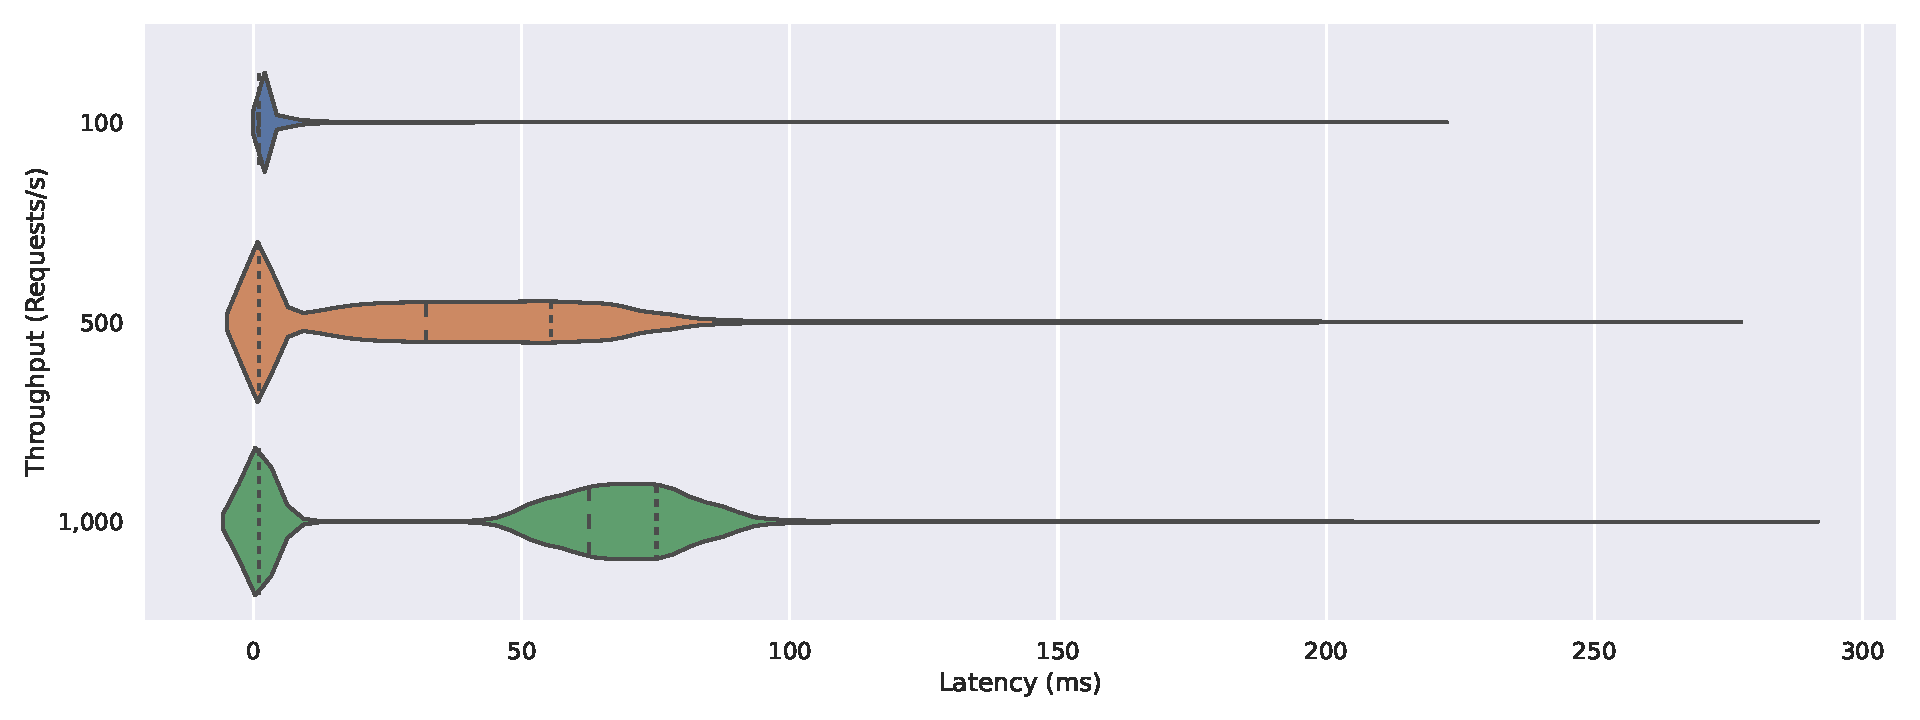
\includegraphics[width=1.2\linewidth]{5_experimental_evaluation/figures/exp-02-bottleneck-traefik.pdf}
    }
    
    \caption[Experiment 2 - Latency distribution of Traefik under varying levels of constant throughput.]{Latency distribution of Traefik under varying levels of constant throughput.}
    
    \label{fig:exp:02:traefik-bottleneck}
\end{figure}

Through the violin plots as depicted in \cref{fig:exp:02:traefik-bottleneck}, we can observe the behaviour and bottlenecks of the system under load in more detail. The first violin plot shows the latency distribution when it is under a constant load of 100 requests per second. From this, we can derive that the system can process this amount and that the distribution of latencies is similar to that of other evaluated \gls{sm} systems as previously seen. The second violin plot, however, shows the system under a constant load of 500 requests per second. This plot shows the first signals of a potential bottleneck in the system. We can observe that the observed latency values have a higher spread and that these values are often an order of magnitude higher, often reaching values well above 50 milliseconds. This provides a sharp contrast with the other systems that we evaluated, which performed significantly better under full or near full load. The third violin plot, however, shows the bottleneck in full effect. This plot depicts the system under a constant throughput of 1000 requests per second, which it was unable to process. This results in the previously observed bimodal distribution of requests latencies. This leads us to our sixth main finding:


\begin{shaded*}
    \noindent
    \textbf{MF6}: 
    Traefik experiences bottlenecking behaviour under a load of approximately 500 requests per second resulting in a bimodal distribution of request latencies.
\end{shaded*}


\subsubsection{Resource Utilization Analysis}
\label{sec:experiments:results:per-experiment:02:resource}


\begin{figure}[t]
\centering
\makebox[\linewidth][c]{
    \begin{subfigure}{.65\textwidth}
      \centering
      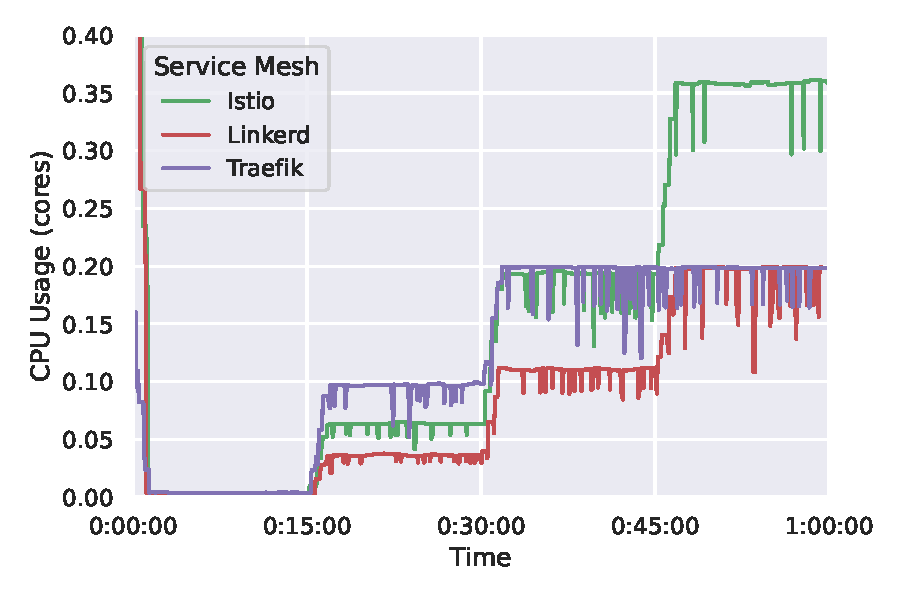
\includegraphics[width=\textwidth]{5_experimental_evaluation/figures/exp-02-cpu-utilization.pdf}
      \caption{CPU Utilization}
      \label{fig:exp:02:resource:cpu}
    \end{subfigure}
    
    
    \begin{subfigure}{.65\textwidth}
      \centering
      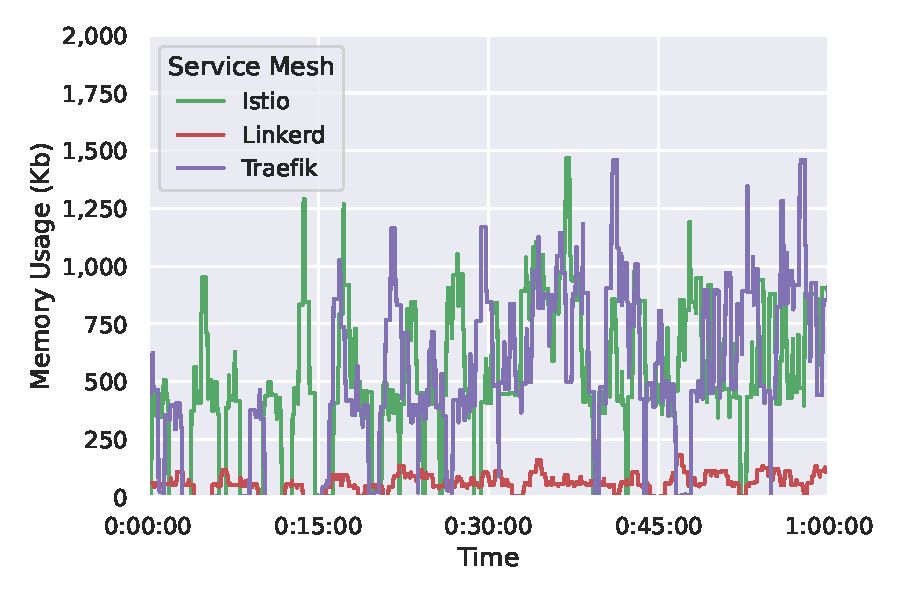
\includegraphics[width=\textwidth]{5_experimental_evaluation/figures/exp-02-memory-utilization.pdf}
      \caption{Memory Utilization}
      \label{fig:exp:02:resource:mem}
    \end{subfigure}
}

\caption[Experiment 2 - Resource utilization for \gls{sm} systems under load.]{Resource utilization for \gls{sm} systems experiencing various levels of constant throughput. The level of throughput is increased at a 15-minute interval, and changes from  1, 100, 500, and 1000 requests per second respectively.}
\label{fig:exp:02:resource-utilization}
\end{figure}

In our first experiment we already took a look at the resource utilization values of various \gls{sm} systems under maximum load. However, those results could not be compared fairly, as they each experienced various levels of load. In this experiment, however, we can evaluate the resource utilization fairly as they are evaluated under similar circumstances. 

In \cref{fig:exp:02:resource-utilization} we present two plots related to the resource consumption of \gls{sm} systems. Both plots can be interpreted similarly. On the y-axis we have the value of interest, which is the CPU utilization as expressed in fractions of a core for the first plot and is the memory utilization expressed in Kb for the second plot. The x-axis presents the time delta of the experiment since the start. It is important to note the labels on the x-axis as these 15-minute intervals represent the time point in which the level of constant throughput was increased. The four intervals represent the constant levels of throughput from 1, 100, 500, and 1000 requests per second respectively (e.g. the interval from 0:30:00 to 0:45:00 represents the systems under a constant load of 500 requests per second). Additionally, the colours of the line represent the various \gls{sm} systems that we evaluated. As previously noted, we are unable to evaluate the actual resource utilization of Cilium as the actual in-kernel proxy is not exposed as a user-space application in the form of a container.

The first plot (\cref{fig:exp:02:resource:cpu}), shows the CPU utilization throughout the experiment for the various \gls{sm} systems. The first thing we can observe the high values at the start of the experiment, these can be explained by the sampling rate used for the time series data which overlaps with the results from the previous experiment. The second thing we can notice is that the line from Traefik does not increase at the 45:00 minute marker. This behaviour falls in line with the previously discussed bottlenecks in our extensive analysis of the bottlenecks of Traefik. Another observation that we can make is that the CPU utilization is relatively stable for all the evaluated systems throughout the duration of the experiment, we can derive this from the lack of extremes and spikes in the presented plot.

More importantly, however, we can observe how the systems scale when the load on these systems is increased. By looking at the first 15-minute interval, we can observe that the proxies require little to no CPU utilization when they experience next to zero load (1 request per second). Interestingly however, is the behaviour when the load is increased to 100 requests per second as it allows us to fairly compare these systems under a similar load. We can observe that the Traefik proxy utilizes the CPU the most, whereas the proxy in the Istio data plane requires just slightly more than half of Traefik's usage. The Linkerd proxy, however, puts the least amount of strain on the CPU requiring less than 5\% of a CPU core at any given time. To analyse how these systems scale we take a closer look at the third and final time intervals. From this, we can observe that the CPU utilization scales linearly with the levels of throughput that a proxy is facing. We can also observe that the proxy empowering the Linkerd \gls{sm} scales significantly better than the one found in Istio. This is exemplified by the fact that Istio under a load of 500 requests per second uses nearly identical amount of CPU resources when Linkerd serves double the number of requests per second. This leads us to a seventh main finding:

\begin{shaded*}
    \noindent
    \textbf{MF7}: 
    There can be a significant difference in the amount of CPU utilization for different \gls{sm} systems under similar levels of load.
\end{shaded*}

The second plot (\cref{fig:exp:02:resource:mem}), shows the CPU utilization throughout the experiment for the various \gls{sm} systems. The first observation that we can make is that the amount of memory consumed for all systems does not seem to vary much across the various levels of throughput. Furthermore, we can observe that the linkerd proxy consumes the least amount of memory whereas Traefik and Istio's data plane proxy seem to consume similar amounts. More importantly, however, is that all the observed values are negligible for most environments. This brings us to our eighth main finding:

\begin{shaded*}
    \noindent
    \textbf{MF8}: 
    The memory footprint of data plane proxies is negligible and does not significantly increase under higher levels of throughput.
\end{shaded*}
